% !TEX root = ../main.tex

\section{Design and implementation}

\subsection{Pre-process data}
\begin{frame}{\insertsubsec}
  \begin{itemize}
    \item Pre-process image data
    \item Pre-process scalar data
    \item Generate pairs for training
  \end{itemize}

  \vspace{.5cm}
  Only 490 of the initial 671 could be used to fit a model because we needed the following 
  requirements:
  \begin{itemize}
    \item CT scan
    \item Tumour annotations
    \item Radiomic features
    \item Clinical information
  \end{itemize}
\end{frame}

\begin{frame}{Image data pre-processing}
  \begin{figure}
    \centering
    \scalebox{.6}{\def\customimage{10em}
\begin{tikzpicture}[node distance = 2]
    \node (P-0) at (0, 0) {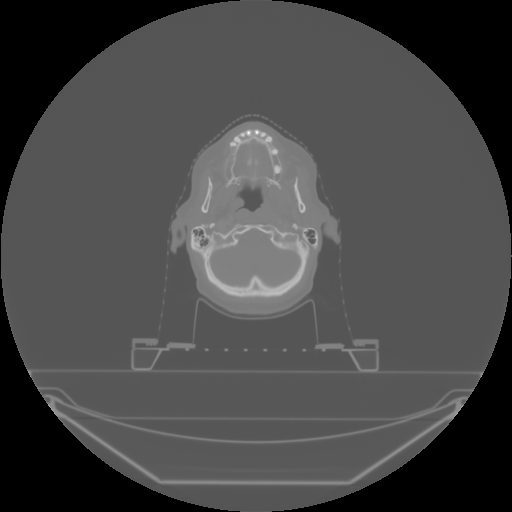
\includegraphics[width=\customimage]{images/preprocess/process_0}};
    \node [below = of P-0] (P-1) {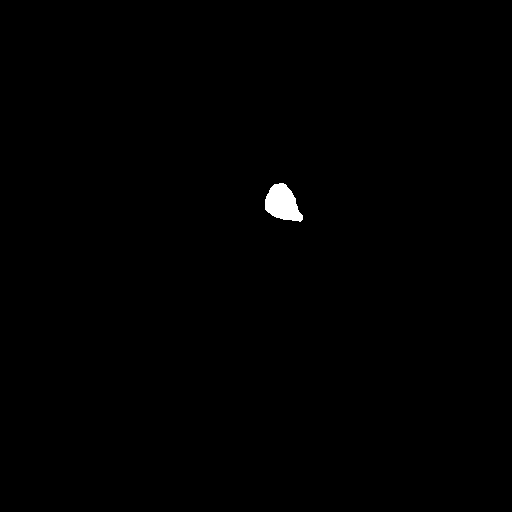
\includegraphics[width=\customimage]{images/preprocess/process_1}};

    \node [below = .2 of P-0] (text-0) {Scan};
    \node [below = .2 of P-1] (text-1) {Mask};
    
    \node [right = of P-1] (P-2-0) {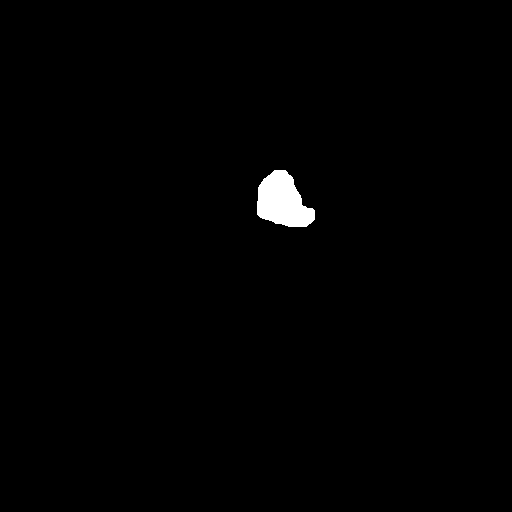
\includegraphics[width=\customimage]{images/preprocess/process_2_0}};
    \node [right = of P-2-0] (P-2-1) {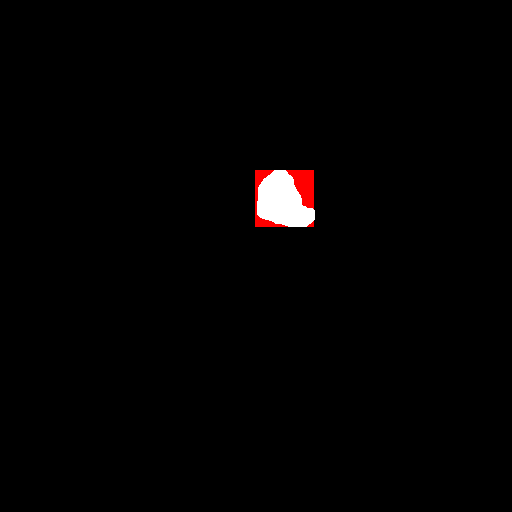
\includegraphics[width=\customimage]{images/preprocess/process_2_1}};
    \node [right = of P-2-1] (P-5) {
\includegraphics[width=\customimage]{images/preprocess/process_5}};
    
    \node [above = of P-2-1] (P-3) {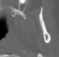
\includegraphics[width=\customimage]{images/preprocess/process_3}};
    \node [right = of P-3] (P-4) {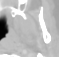
\includegraphics[width=\customimage]{images/preprocess/process_4}};

    \node [right = .5 of P-5, circle, draw] (prod) { \Large \( \times \) };
    
    \node [below = of P-5] (P-6) {
\includegraphics[width=\customimage]{images/preprocess/process_6}};
    \node [left = of P-6] (P-7) {
\includegraphics[width=\customimage]{images/preprocess/process_7}};
    \node [left = of P-7] (P-8) {
\includegraphics[width=\customimage]{images/preprocess/process_8}};

    \node [below = .2 of P-6] { \( 59 \times 57 \) px};
    \node [below = .2 of P-7] { \( 64 \times 64 \) px};
    \node [below = .2 of P-8] { \( 64 \times 64 \) px};

    \draw [-latex] (P-0) -- (P-3);
    \draw [-latex] (P-3) -- (P-4) node[midway, below, align=center] {Remove \\ extreme \\ values};
    \draw [-latex] (P-4) -| (prod);

    \draw [-latex] (P-1) -- (P-2-0) node[midway, below, align=center] {Gaussian \\ filter};
    \draw [-latex] (P-2-0) -- (P-2-1) node[midway, below, align=center] {Bounding \\ box};
    \draw [-latex] (P-2-1) -- (P-3) node[midway, right, align=center] {Slice};
    \draw [-latex] (P-2-1) -- (P-5) node[midway, below, align=center] {Slice};
    \draw [-latex] (P-5) -- (prod);

    \draw [-latex] (prod) |- (P-6) node[near end, below, align=center] {Apply \\ mask};
    \draw [-latex] (P-6) -- (P-7) node[midway, below, align=center] {
        Resize \\ \( 64 \times 64 \times 64 \)
    };

    \draw [-latex] (P-7) -- (P-8) node[midway, below, align=center] {Normalize};

\end{tikzpicture}}
    \caption{Image data pre-processing}
  \end{figure}
\end{frame}

\begin{frame}{Scalar data pre-processing}
  \begin{itemize}
    \item Clinical information
    \begin{itemize}
      \item Patient's ID
      \item Age
      \item Sex
      \item Survival event
      \item Survival time
    \end{itemize}
    \item Radiomic features, up to 725
    \begin{itemize}
      \item Tumour shape
      \item Intensity
      \item Volume
      \item ...
    \end{itemize}
  \end{itemize}
\end{frame}
\begin{frame}
  \begin{figure}
    \centering
    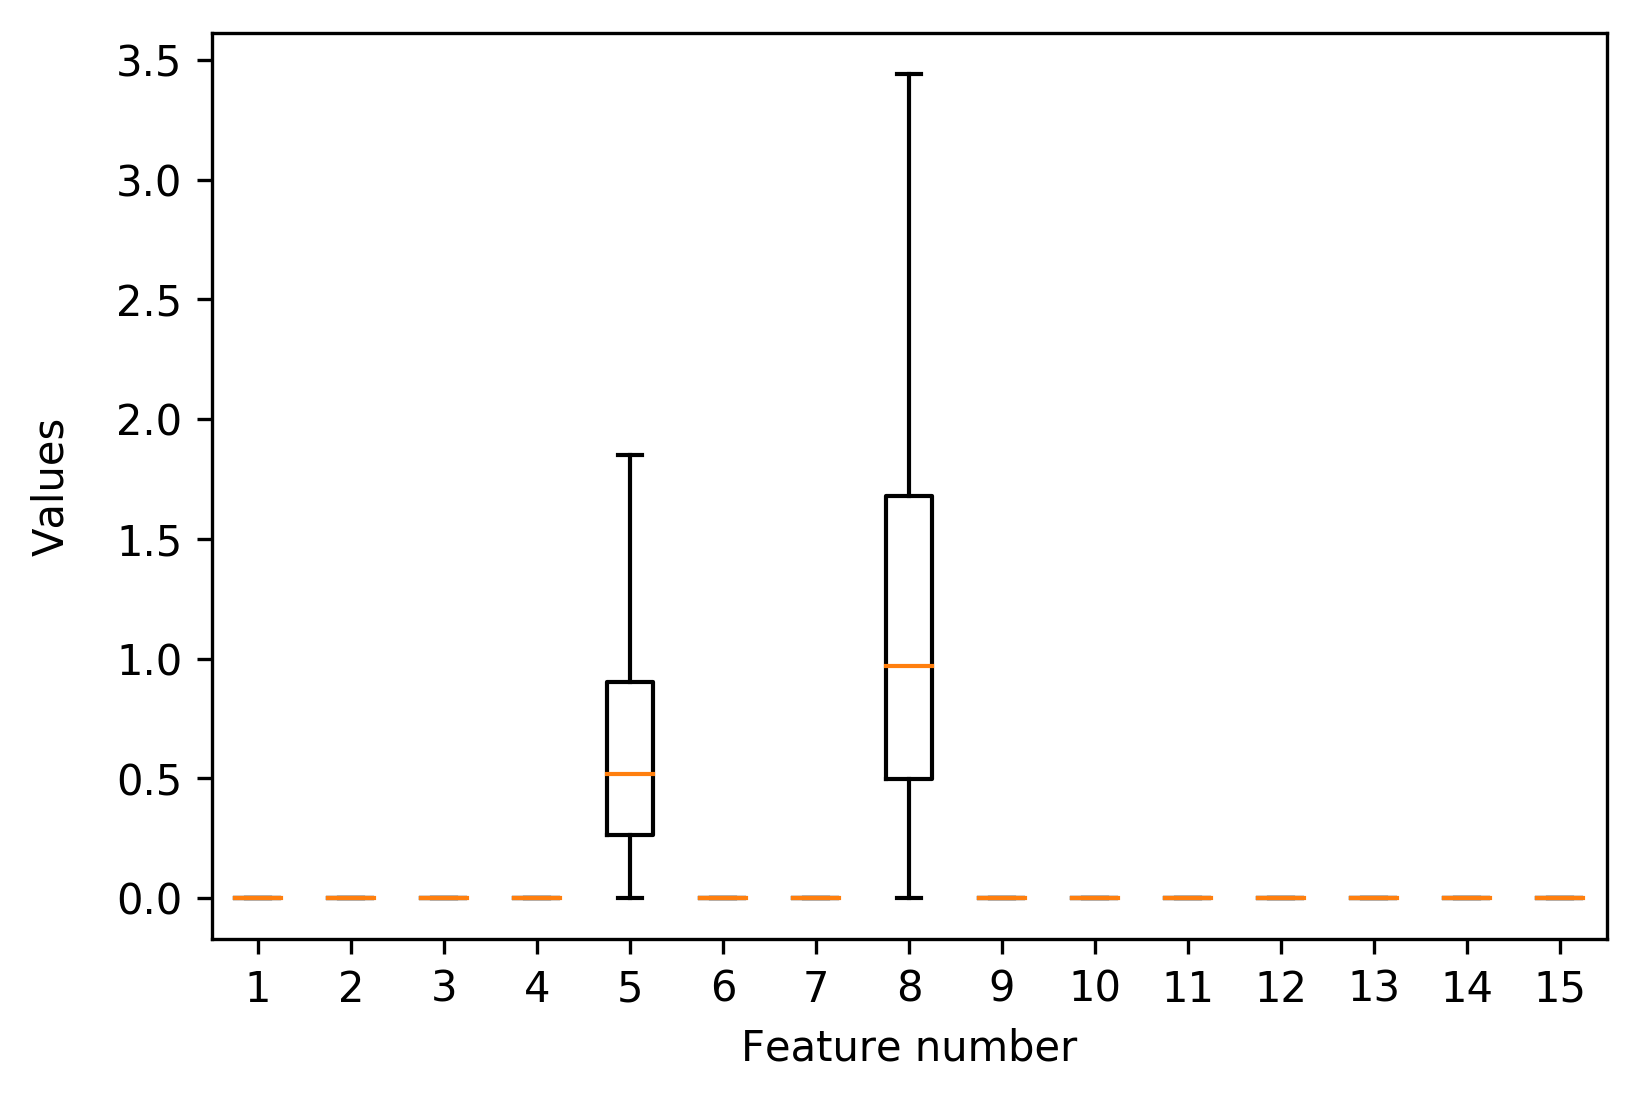
\includegraphics[width=\textwidth]{images/features_original}
    \caption{Features before normalization}
  \end{figure}
\end{frame}
\begin{frame}
  \begin{figure}
    \centering
    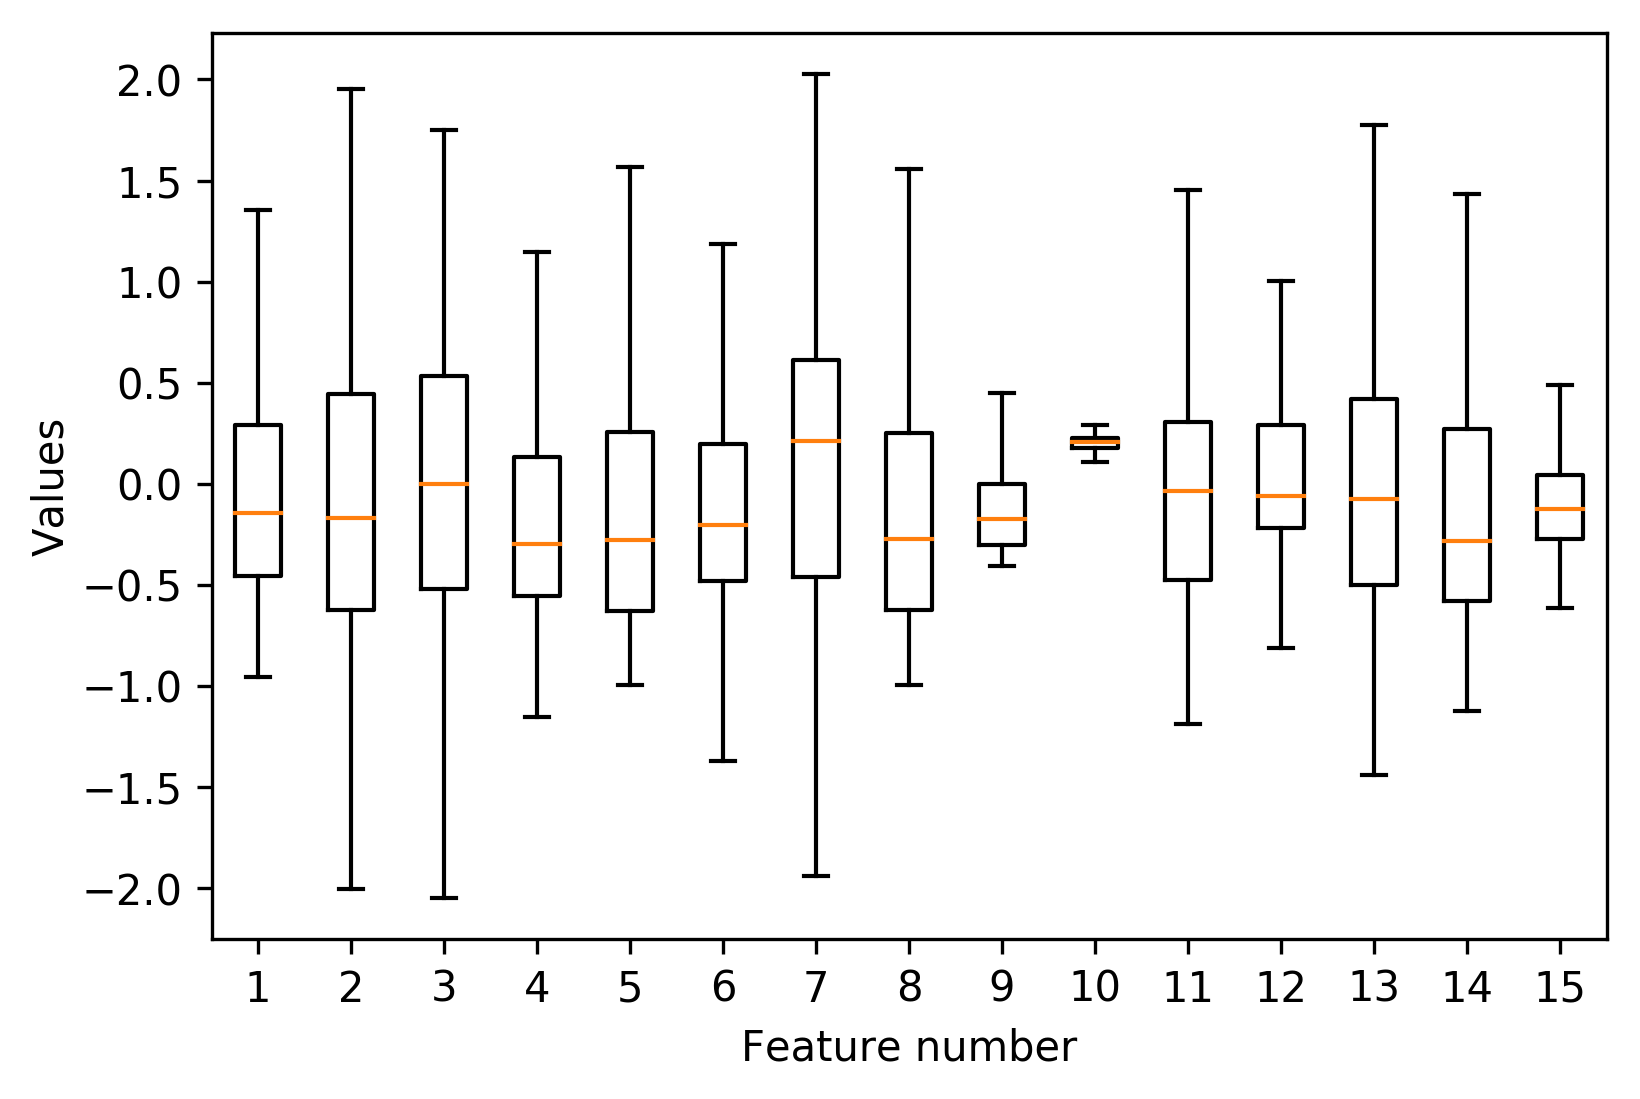
\includegraphics[width=\textwidth]{images/features_normalized}
    \caption{Features after normalization}
  \end{figure}
\end{frame}

\begin{frame}{Pair generation}
  
  \begin{figure}
    \centering
    \scalebox{.7}{\def\customimage{5em}
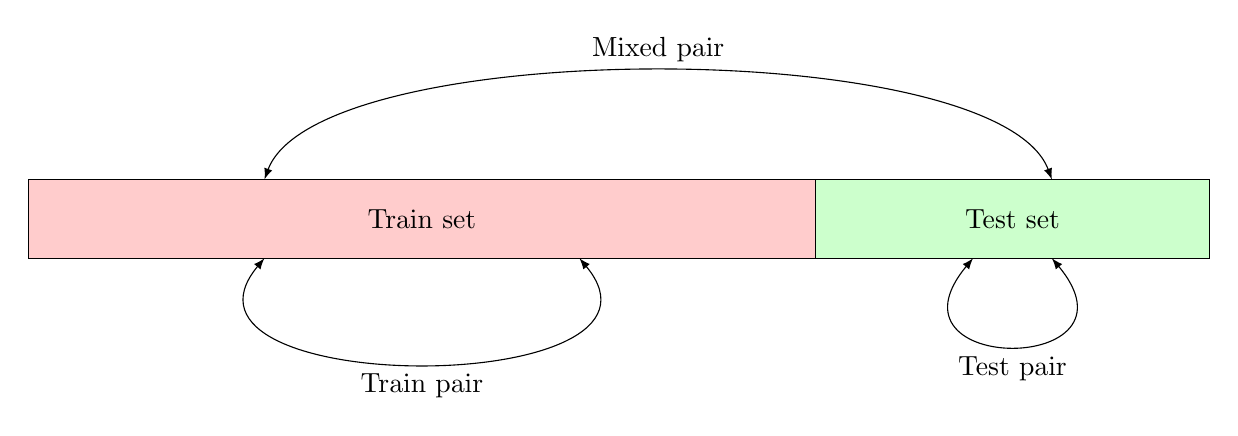
\begin{tikzpicture}
    
    \draw [fill = red!20] (0, 0) rectangle (10, 1);
    \draw [fill = green!20] (10, 0) rectangle (15, 1);

    \node at (5, .5) {Train set};
    \node at (12.5, .5) {Test set};

    \draw [bend right=130, latex-latex, looseness=1.5] (3, 0) to node [midway, below] {Train pair} (7, 0);
    \draw [bend right=130, latex-latex, looseness=5] (12, 0) to node [midway, below] {Test pair} (13, 0);
    \draw [bend left=70, latex-latex, looseness=.5] (3, 1) to node [midway, above] {Mixed pair} (13, 1);
\end{tikzpicture}}
    \caption{Types of pairs generated from train and test sets}
  \end{figure}

  \begin{block}{Conditions}
    \begin{itemize}
      \item Both of them are uncensored \( E_A = E_B = 1 \)
      \item The uncensored time of one is smaller than the censored time of the other
            \( T_A < T_B | E_A = 1; E_B = 0 \)
    \end{itemize}
  \end{block}
\end{frame}

\subsection{Create basic siamese model}
\begin{frame}{\insertsubsec}
  Step required from a software engineering perspective. Future models should implement the 
  \( \operatorname{sister}(x) \) function.
  \begin{figure}
    \scalebox{.7}{\begin{tikzpicture}
  \tikzstyle{module}=[rounded corners, draw]
  \tikzstyle{sister}=[module, fill=cyan!20]

  \node [sister] (S-1) at (0, 0) {Sister Network \#1};
  \node [below = .5 of S-1] (aux-1) {};
  \node [sister, below = .5 of aux-1] (S-2) {Sister Network \#2};

  \node [left = of S-1] (I-1) {Input 1};
  \node [left = of S-2] (I-2) {Input 2};

  \node [module, right = of aux-1, fill=red!20] (M-1) {Contrastive Loss};

  \node [right = of M-1] (O-1) {Output};

  \draw [-latex] (I-1) -- (S-1);
  \draw [-latex] (I-2) -- (S-2);

  \draw [-latex] (S-1) -- (M-1);
  \draw [-latex] (S-2) -- (M-1);

  \draw [-latex] (M-1) -- (O-1);

  \draw [latex-latex] (S-1) -- (S-2) node[midway, left] {Weights};
\end{tikzpicture}}
    \caption{Siamese network illustration}
  \end{figure}
\end{frame}
\begin{frame}
  \begin{align*}
    \bm{O}_A &= \operatorname{sister}(\bm{X}_A) \\
    \bm{O}_B &= \operatorname{sister}(\bm{X}_B) \\
    \sigma(x) &= \frac{1}{1 + \exp(-x)} \\
    \hat{y} &= \sigma(||\bm{O}_B||_2 - ||\bm{O}_A||_2) 
  \end{align*}

  \[
    \mathcal{L}(\bm{y}, \hat{\bm{y}}) = -\frac{1}{N} \sum_{i = 1}^{N}
    (1 - y_i)\log(1 - \hat{y}_i) + y_i\log(\hat{y}_i)
  \]

  \[
    C(\bm{y}, \hat{\bm{y}}) = \mathcal{L}(\bm{y}, \hat{\bm{y}}) + 
    ||\bm{w}||_2
  \]
\end{frame}

\subsection{Build volume only model}
\begin{frame}{\insertsubsec}
  Very simple model to have a baseline

  \[
    \operatorname{sister}(\bm{X}) = w\cdot X_{\text{scalar}_{26}} + b
  \]
\end{frame}
\begin{frame}
  Parameters:
  \begin{itemize}
    \item Learning rate: 0,05
    \item Number of epochs: 200
    \item Batch size: The whole dataset
  \end{itemize}

  Previous state-of-the-art CI was 0,628.

  \begin{table}
    \centering
    \begin{tabular}{|c||c|c|c||c|c|c|}
      \cline{2-7}
      \multicolumn{1}{c|}{} & \multicolumn{3}{|c||}{\textbf{Pairs}} & 
      \multicolumn{3}{c|}{\textbf{Concordance Index}} \\
      \hline
      \textbf{Fold} & \textbf{Mixed} & \textbf{Train} & \textbf{Test} 
      & \textbf{Mixed} & \textbf{Train} & \textbf{Test} \\
      \hhline{=======}
      0 & 16.359 & 46.804 & 5.330 & 0,627 & 0,634 & 0,639 \\
      1 & 16.359 & 46.957 & 5.278 & 0,629 & 0,635 & 0,63 \\
      2 & 16.348 & 47.577 & 5.084 & 0,636 & 0,627 & 0,661 \\
      3 & 16.348 & 47.274 & 5.176 & 0,618 & 0,644 & 0,6 \\
      \hhline{=======}
      \textbf{Total} & 65.414 & 188.612 & 20.868 & 0,627 & 0,635 & 0,632 \\
      \hline
    \end{tabular}
  
    \caption[Volume Only 4-CV results]{
      Results for volume only model using 4-CV \label{tab:results-volume-4CV}
    }
  \end{table}
\end{frame}

\begin{frame}
  \begin{figure}
    \centering
    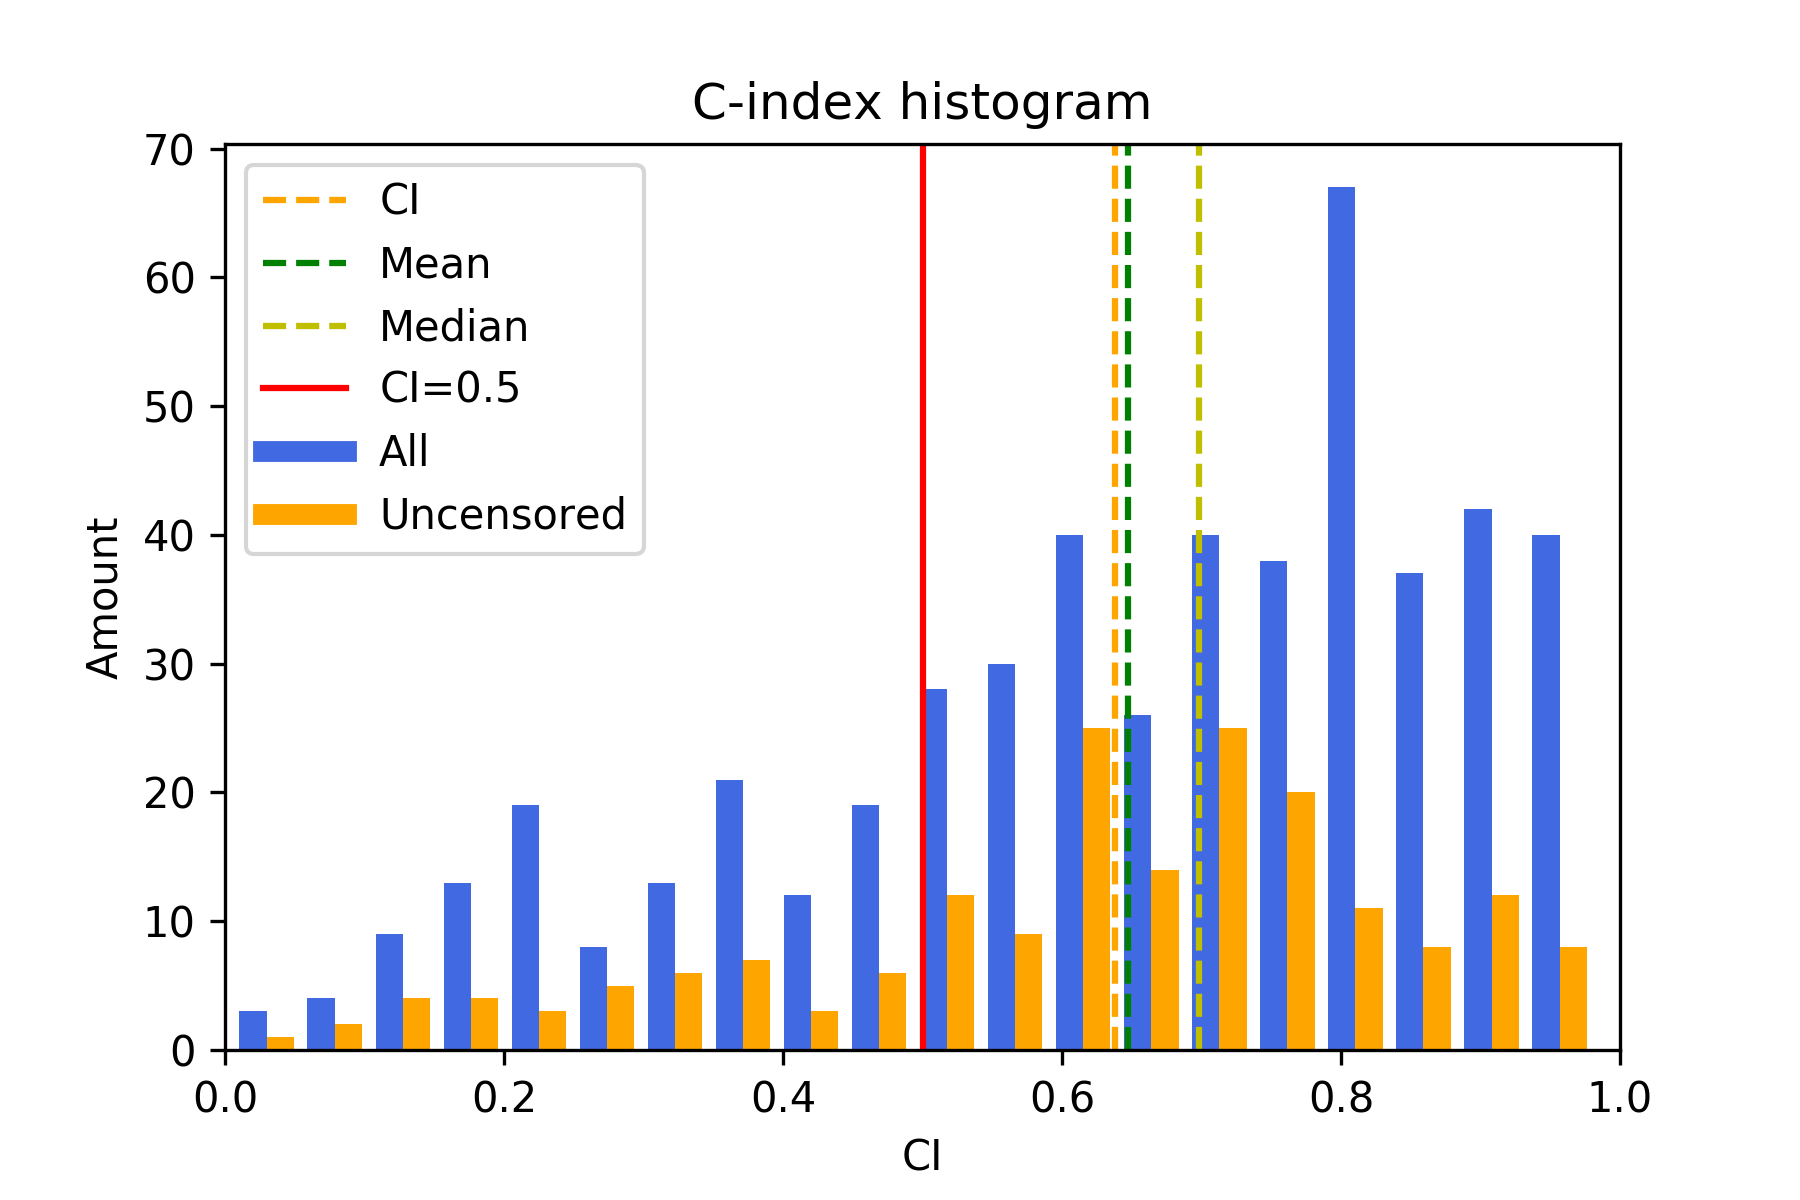
\includegraphics[width=.8\textwidth]{images/results/c-index_volume}
    \caption[LOOCV volume only model results]{
      Volume only model results using LOOCV \label{fig:results-volume-LOOCV}
    }
  \end{figure}
  LOOCV CI is 0,627.
\end{frame}

\subsection{Build shallow siamese network}
\begin{frame}{\insertsubsec}
  \begin{figure}
    \centering
    \scalebox{.7}{
\begin{tikzpicture}[every node/.style={scale=.8}]

  \tikzstyle{module}=[rounded corners, draw, align=center]
  \tikzstyle{FC}=[module, fill=green!30]
  \tikzstyle{conv}=[module, fill=orange!30]
  \tikzstyle{io}=[module, fill=purple!30]
  
  
  \node [io] (image) {Image};
  \node [conv, below = of image] (CNN-1) at (0, 0) {
    Convolution 1 \\ 
    \( 30 @ 3 \times 3 \times 3 \) \\
    Stride = 2
  };
  \node [conv, below = of CNN-1] (CNN-2) {
    Convolution 2 \\
    \( 30 @ 3 \times 3 \times 3 \) \\
    Stride = 2
  };
  \node [conv, below = of CNN-2] (CNN-3) {
    Convolution 3 \\
    \( 40 @ 3 \times 3 \times 3 \)
  };
  \node [conv, below = of CNN-3] (CNN-4) {
    Convolution 4 \\
    \( 40 @ 3 \times 3 \times 3 \)
  };
  \node [conv, below = of CNN-4] (CNN-5) {
    Convolution 5 \\
    \( 50 @ 3 \times 3 \times 3 \)
  };

  \node [right = 5 of image] (aux) {};
  \node [io, right = of aux] (scalar) {Scalar};

  \node [FC, below = of aux] (con) {Concatenate + \\ flatten};
  \node [left = of con] (aux-2) {};
  \node [FC, below = of con] (FC-1) {FC \\ 8000 units};
  \node [FC, below = of FC-1] (FC-2) {FC \\ 1000 units};
  \node [FC, below = of FC-2] (FC-3) {FC \\ 10 units};

  \node [io, below = of FC-3] (out) {Sister out};
  
  \draw [-latex] (image) -- (CNN-1) node[midway, right] {\( 64 \times 64 \times 64 \times 1 \)};
  \draw [-latex] (CNN-1) -- (CNN-2) node[midway, right] {\( 31 \times 31 \times 31 \times 30 \)};
  \draw [-latex] (CNN-2) -- (CNN-3) node[midway, right] {\( 15 \times 15 \times 15 \times 40 \)};
  \draw [-latex] (CNN-3) -- (CNN-4) node[midway, right] {\( 13 \times 13 \times 13 \times 40 \)};
  \draw [-latex] (CNN-4) -- (CNN-5) node[midway, right] {\( 11 \times 11 \times 11 \times 40 \)};

  \draw (CNN-5) -| (aux-2.center)  node[pos=.3, below] {\( 9 \times 9 \times 9 \times 50 \)};
  \draw [-latex] (aux-2.center) |- (con);
  \draw [-latex] (scalar) |- (con) node[pos=.15, left] {\( 725 \)};
  
  \draw [-latex] (con) -- (FC-1) node[midway, right] {\( 37.175 \)};
  \draw [-latex] (FC-1) -- (FC-2) node[midway, right] {\( 8000 \)};
  \draw [-latex] (FC-2) -- (FC-3) node[midway, right] {\( 1000 \)};
  \draw [-latex] (FC-3) -- (out) node[midway, right] {\( 10 \)};
\end{tikzpicture}


}
    \caption{Shallow siamese sister's network illustration \label{fig:shallow-implement}}
  \end{figure}
\end{frame}

\begin{frame}
  \begin{itemize}
    \item Learning rate: 0,05
    \item Number of epochs: 200
    \item Batch size: The whole dataset
  \end{itemize}

  \begin{table}
    \centering
    \begin{tabular}{|c||c|c|c||c|c|c|}
      \cline{2-7}
      \multicolumn{1}{c|}{} & \multicolumn{3}{|c||}{\textbf{Pairs}} & 
      \multicolumn{3}{c|}{\textbf{Concordance Index}} \\
      \hline
      \textbf{Fold} & \textbf{Mixed} & \textbf{Train} & \textbf{Test} 
      & \textbf{Mixed} & \textbf{Train} & \textbf{Test} \\
      \hhline{=======}
      0 & 16.359 & 46.804 & 5.330 & 0,627 & 0,634 & 0,639 \\
      1 & 16.359 & 46.957 & 5.278 & 0,629 & 0,635 & 0,63 \\
      2 & 16.348 & 47.577 & 5.084 & 0,636 & 0,627 & 0,661 \\
      3 & 16.348 & 47.274 & 5.176 & 0,618 & 0,644 & 0,6 \\
      \hhline{=======}
      \textbf{Total} & 65.414 & 188.612 & 20.868 & 0,627 & 0,635 & 0,632 \\
      \hline
    \end{tabular}
  
    \caption[Volume Only 4-CV results]{
      Results for volume only model using 4-CV \label{tab:results-volume-4CV}
    }
  \end{table}
\end{frame}

\subsection{Build scalar only siamese network}
\begin{frame}{\insertsubsec}
  \begin{figure}
    \centering
    
\begin{tikzpicture}[every node/.style={scale=.8}]

  \tikzstyle{module}=[rounded corners, draw, align=center]
  \tikzstyle{FC}=[module, fill=green!30]
  \tikzstyle{conv}=[module, fill=orange!30]
  \tikzstyle{io}=[module, fill=purple!30]

  \node [io] (scalar) {Scalar};

  \node [FC, right = of scalar] (FC-1) {FC \\ 500 units \\ tanh};
  \node [conv, right = of FC-1] (D-1) {Dropout \\ 20\%};
  \node [FC, right = of D-1] (FC-2) {FC \\ 200 units \\ tanh};
  \node [conv, right = of FC-2] (D-2) {Dropout \\ 20\%};

  \node [FC, below = of FC-1] (FC-3) {FC \\ 50 units \\ tanh};
  \node [conv, right = of FC-3] (D-3) {Dropout \\ 20\%};
  \node (aux) at ($(FC-3)!0.5!(FC-1)$) {};
  \node [FC, right = of D-3] (FC-4) {FC \\ 10 units \\ ReLu};


  \node [io, right = of FC-4] (out) {Sister out};
  \draw [-latex] (scalar) -- (FC-1) node[midway, below] {\( 725 \)};

  \draw [-latex] (FC-1) -- (D-1) node[midway, below] {\( 500 \)};
  \draw [-latex] (D-1) -- (FC-2) node[midway, below] {\( 500 \)};
  \draw [-latex] (FC-2) -- (D-2) node[midway, below] {\( 200 \)};
  
  \draw [-latex] (D-2) |- node[pos=.75, below]{\( 200 \)} (aux) -| (FC-3);
  \draw [-latex] (FC-3) -- (D-3) node[midway, below] {\( 50 \)};
  \draw [-latex] (D-3) -- (FC-4) node[midway, below] {\( 50 \)};
  \draw [-latex] (FC-4) -- (out) node[midway, below] {\( 10 \)};

  % \draw [-latex] (FC-3) -- (out) node[midway, below] {\( 10 \)};
\end{tikzpicture}



    \caption{Scalar siamese network illustration \label{fig:scalar-implement}}
  \end{figure}
\end{frame}

\begin{frame}
  \begin{itemize}
    \item Learning rate: 0,001
    \item Regularization factor: 0,01
    \item Dropout probability: 20\%
    \item Number of epochs: 1000
    \item Batch size: The whole dataset
  \end{itemize}

  \begin{table}
    \centering
    \begin{tabular}{|c||c|c|c||c|c|c|}
      \cline{2-7}
      \multicolumn{1}{c|}{} & \multicolumn{3}{|c||}{\textbf{Pairs}} & 
      \multicolumn{3}{c|}{\textbf{Concordance Index}} \\
      \hline
      \textbf{Fold} & \textbf{Mixed} & \textbf{Train} & \textbf{Test} & 
      \textbf{Mixed} & \textbf{Train} & \textbf{Test} \\
      \hhline{=======}
      0 & 16.359 & 46.804 & 5.330 & 0,728 & 0,915 & 0,543 \\
      1 & 16.359 & 46.957 & 5.278 & 0,809 & 0,927 & 0,64 \\
      2 & 16.348 & 47.577 & 5.084 & 0,751 & 0,91 & 0,675 \\
      3 & 16.348 & 47.274 & 5.176 & 0,766 & 0,919 & 0,624 \\
      \hhline{=======}
      \textbf{Total} & 65.414 & 188.612 & 20.868 & 0,764 & 0,918 & 0,62   \\
      \hline
    \end{tabular}
  
    \caption[Scalar Only 4-CV results]{
      Results for scalar only model using 4-CV \label{tab:results-scalar-4CV}
    }
  \end{table}
\end{frame}

\begin{frame}
  \begin{figure}
    \centering
    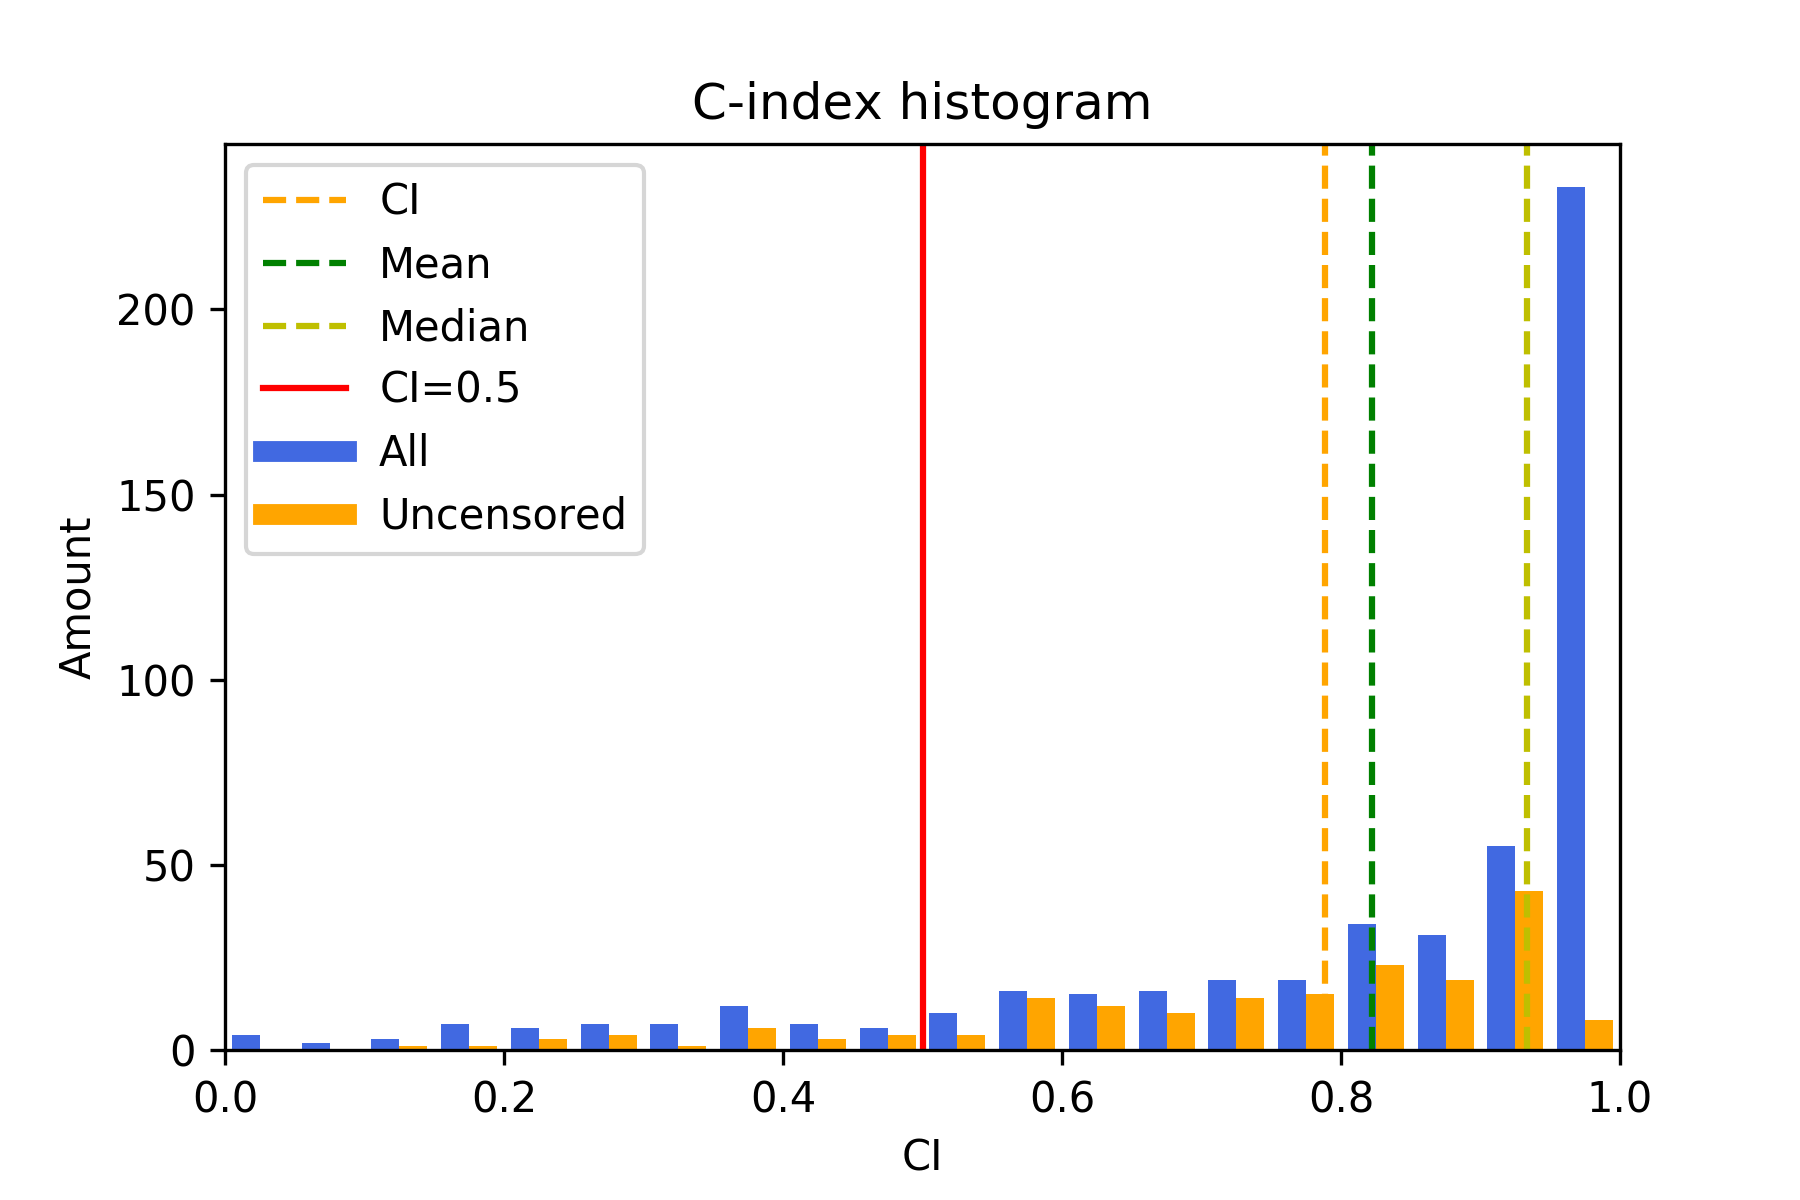
\includegraphics[width=.8\textwidth]{images/results/c-index_scalar}
    \caption[LOOCV scalar only model results]{
      Scalar only model results using LOOCV \label{fig:results-scalar-LOOCV}
    }
  \end{figure}

  Final CI is 0,771
\end{frame}

\subsection{Build deep siamese network}
\begin{frame}{\insertsubsec}
  \begin{figure}
    \centering
    \scalebox{.7}{\input{drawings/residual_general.tikz.tex}}
    \caption[Deep siamese network main structure]{
      Deep siamese network main structure \label{fig:residual-general}
    }
  \end{figure}
\end{frame}

\begin{frame}
  \begin{itemize}
    \item Learning rate: 0,001
    \item Regularization factor: 0,01
    \item Dropout probability: 0,2/1
    \item Number of epochs: 15
    \item Batch size: 20
  \end{itemize}

  \begin{table}
    \centering
    \begin{tabular}{|c||c|c|c||c|c|c|}
      \cline{2-7}
      \multicolumn{1}{c|}{} & \multicolumn{3}{|c||}{\textbf{Pairs}} & 
      \multicolumn{3}{c|}{\textbf{Concordance Index}} \\
      \hline
      \textbf{Fold} & \textbf{Mixed} & \textbf{Train} & \textbf{Test} & 
      \textbf{Mixed} & \textbf{Train} & \textbf{Test} \\
      \hhline{=======}
      0 & 65.436 & 187.216 & 21.320 & 0,765 & 0,812 & 0,814 \\
      1 & 65.436 & 187.828 & 21.112 & 0,821 & 0,813 & 0,813 \\
      2 & 65.392 & 190.308 & 20.336 & 0,427 & 0,431 & 0,387 \\
      3 & 65.392 & 189.096 & 20.704 & 0,389 & 0,359 & 0,428 \\
      \hhline{=======}
      \textbf{Total} & 261.656 & 754.448 & 83.472 & 0,601 & 0,603 & 0,614 \\
      \hline
    \end{tabular}
  
    \caption[Residual 4-CV results]{
      Results for residual model using 4-CV \label{tab:results-residual-4CV}
    }
  \end{table}
\end{frame}